% # COPYRIGHT:
%
% Copyright (C) 2011 Jeremiah Mahler <jmmahler@gmail.com>.
% Permission is granted to copy, distribute and/or modify this document
% under the terms of the GNU Free Documentation License, Version 1.3
% or any later version published by the Free Software Foundation;
% with no Invariant Sections, no Front-Cover Texts, and no Back-Cover Texts.
% A copy of the license is included in the file "fdl-1.3.txt".
%
\documentclass[12pt]{article}
%\usepackage{mslapa}
\usepackage{hyperref}
\usepackage{amsmath}
\usepackage{graphicx}
\usepackage{ulem}
\usepackage{vmargin}
\usepackage{tabularx}
\usepackage{sectsty}
\usepackage{pbox}
\usepackage{bigstrut}
\usepackage{enumerate}
\usepackage{parskip} % add spaces between paragraphs
\input kvmacros % Karnaugh Maps and Veitch charts
%\usepackage{cleveref}
\setpapersize{USletter}
%\setpapersize{A4}
%\setmarginsrb{<leftmargin>}{<topmargin>}{<rightmargin>}{<bottommargin>}
% {<headheight>}{<headsep>}{<footheight>}{<footskip>}
%\setmarginsrb{1.25in}{1.0in}{1.0in}{1.0in}{0in}{0.25in}{0in}{0.20in}
\setmarginsrb{1.0in}{1.0in}{1.0in}{1.0in}{0in}{0.25in}{0in}{0.20in}
\sectionfont{\normalsize}
\subsectionfont{\normalsize}
% configure \bigstrut size
% This configures spacing above and below rows in a tabularx.
%\renewcommand{\bigstrutjot}{6pt}
\renewcommand{\bigstrutjot}{2.0\jot}
\setlength{\parindent}{0in}
\raggedright
\begin{document}

% {{{ Cover Page
\centerline{\bf EECE 144}
\centerline{\bf Fall 2011}
\centerline{\bf}
\centerline{\bf Lab Report \#7}
\centerline{\bf Section 4}
\centerline{\bf 10/19/2011}
% signature area
\begin{center}
\begin{tabularx}{\textwidth}[b]{X l l}
Submitted by: Marvanee Johnson & & \\
Signature & Printed Name & Date \\
\hline
\multicolumn{1}{|X|}{} & \multicolumn{1}{|l|}{\bigstrut \bf Jeremiah Mahler} & \multicolumn{1}{|l|}{\bf Oct 19, 2011} \\
\hline
\multicolumn{1}{|X|}{} & \multicolumn{1}{|l|}{\bigstrut \bf Marvanee Johnson} & \multicolumn{1}{|l|}{\bf Oct 19, 2011} \\
\hline
\end{tabularx}
\end{center}
% }}}

\section{Description/Objectives}
% description
The purpose of this lab is to find the min SOP expressions of equations J \& K using a minimal amount of gates and to build a circut combining the two equations using only two input gates.
(Equation \ref{eq:Jcsop} and \ref{eq:Kcsop}).
\begin{align}
J(w, x, y, z) &= \sum m(1,3,9,11,12,13,14,15) \label{eq:Jcsop} \\
K(w, x, y, z) &= \sum m(0,1,3,12,14) \label{eq:Kcsop}
\end{align}
\section{Procedure}
\label{sec:procedure}
The first step in accomplishing this task was to create seperate Karnaugh Map for expressions J \& K in order to find the min SOPs of the equations and to determin the number of gates needed to implement each equation seperately. The next step was to jointly optimaize the two equations through the use Karnaugh Maps to produce a circut using the minimum number of gates. Lastly, we used the Truth table in order to test and verify the funtionality of the curcuit.
(Table \ref{tbl:tt})
\begin{table}[htb]
\begin{center}
\begin{tabular}{lr}
\begin{tabular}[t]{r|cccc|c|c}
Index&$w$&$x$&$y$&$z$&$J$&$K$\\
\hline
0 &0&0&0&0 &0 &1\\
1 &0&0&0&1 &1 &1\\
2 &0&0&1&0 &0 &0\\
3 &0&0&1&1 &1 &1\\
4 &0&1&0&0 &0 &0\\
5 &0&1&0&1 &0 &0\\
6 &0&1&1&0 &0 &0\\
7 &0&1&1&1 &0 &0\\
8 &1&0&0&0 &0 &0\\
9 &1&0&0&1 &1 &0\\
10 &1&0&1&0 &0 &0\\
11 &1&0&1&1 &1 &0\\
12 &1&1&0&0 &1 &1\\
13 &1&1&0&1 &1 &0\\
14 &1&1&1&0 &1 &1\\
15 &1&1&1&1 &1 &0\\
\end{tabular}
\end{tabular}
\end{center}
\caption{Truth table of functions $J$ and $K$.}
\label{tbl:tt}
\end{table}
The minimal SOP expression for $J$ was found by the use of a Karnaugh Map.
(Figure \ref{fig:Jmap})
(Equation \ref{eq:Jsop}).
\begin{equation}
J = w x + x' z \label{eq:Jsop}
\end{equation}
\begin{figure}[!hbt]
\begin{center}
\karnaughmap{4}{$J(w,x,y,z)$:}{wxyz}{0101000001011111}{}
\end{center}
\caption{Karnaugh map of function $J$ (Equation \ref{eq:Jcsop}).}
\label{fig:Jmap}
\end{figure}
The minimal SOP expression for $K$ was found by the use of a Karnaugh Map.
(Figure \ref{fig:Kmap})
(Equation \ref{eq:Ksop}).
\begin{figure}[!hbt]
\begin{center}
\karnaughmap{4}{$K(w,x,y,z)$:}{wxyz}{1101000000001010}{}
\end{center}
\caption{Karnaugh map of function $K$ (Equation \ref{eq:Kcsop}).}
\label{fig:Kmap}
\end{figure}
\begin{equation}
K = w'x'y' + w'x'z + wxz' \label{eq:Ksop}
\end{equation}
Firgure 1 shows the Karnaugh map used for equation J in order to determine the number of gates and gate inputs needed
A total of 4 gates would be need to implement expression $J$?
(Figure \ref{fig:Jminsop-01})
\begin{figure}[htb]
\center
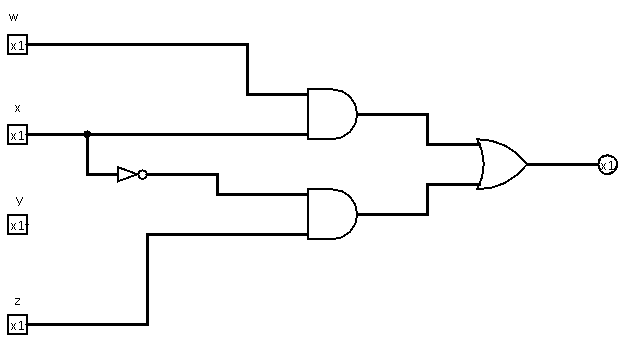
\includegraphics[scale=0.5]{Jminsop-01}
\caption{Circuit diagram of the minimal SOP solution of $J$.}
\label{fig:Jminsop-01}
\end{figure}
Firgure 4 shows the Karnaugh map used for equation K in order to determine the number of gates and gate inputs needed
A total of 8 gates would be need to implement expression $J$?
(Figure \ref{fig:Kminsop-01})
\begin{figure}[!htb]
\center
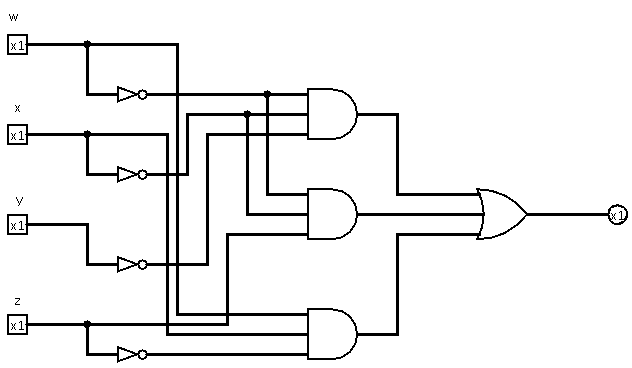
\includegraphics[scale=0.5]{Kminsop-01}
\caption{Circuit diagram of the minimal SOP solution of $K$.}
\label{fig:Kminsop-01}
\end{figure}
TODO: What about the version $K$ limited to 2 input gates?
(Figure \ref{fig:Kminsop-02})
\begin{figure}[!htb]
\center
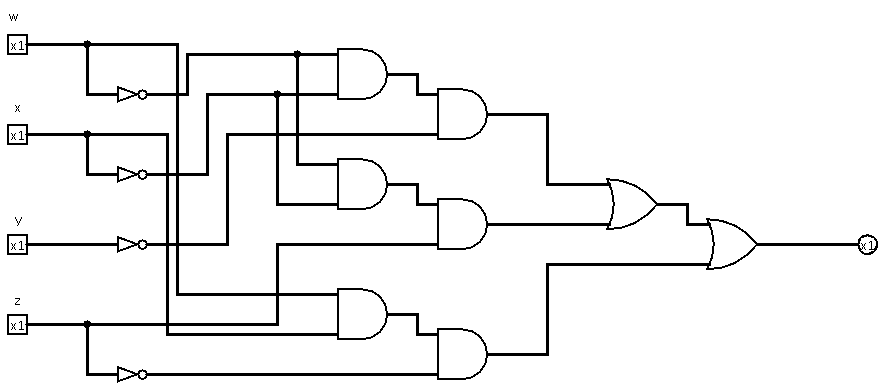
\includegraphics[scale=0.5]{Kminsop-02}
\caption{Circuit diagram of the minimal SOP solution of $K$ when limited to two input gates.}
\label{fig:Kminsop-02}
\end{figure}
\clearpage
A jointly optimized solution of $J$ and $K$ is created by combining shared term used by both SOP espressions of J and K.
(Figure \ref{fig:JKjointkmap})
(Equation \ref{eq:JKjoint})
\begin{align}
J &= w'x'z + wxz' + wz \notag \\
K &= w'x'z + wxz' + w'x'y' \label{eq:JKjoint}
\end{align}
\begin{figure}[!htb]
\center
%\karnaughmap{4}{$J(w,x,y,z)$:}{wxyz}{0101000001011111}{}
%\karnaughmap{4}{$K(w,x,y,z)$:}{wxyz}{1101000000001010}{}
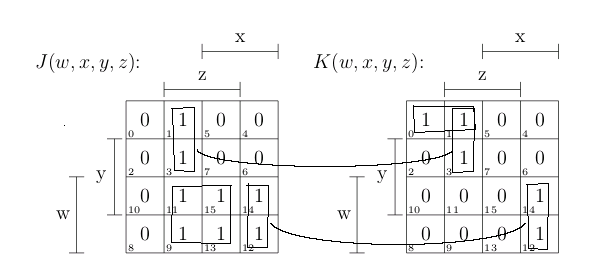
\includegraphics[scale=0.60]{JKkmap-01}
\caption{Jointly optimized Karnaugh maps for $J$ and $K$.}
\label{fig:JKjointkmap}
\end{figure}
15 gates, and 7 inputs is the result of J and K joint solution
(Figure \ref{fig:JKjointcircuit}).
\begin{figure}[!htb]
\center
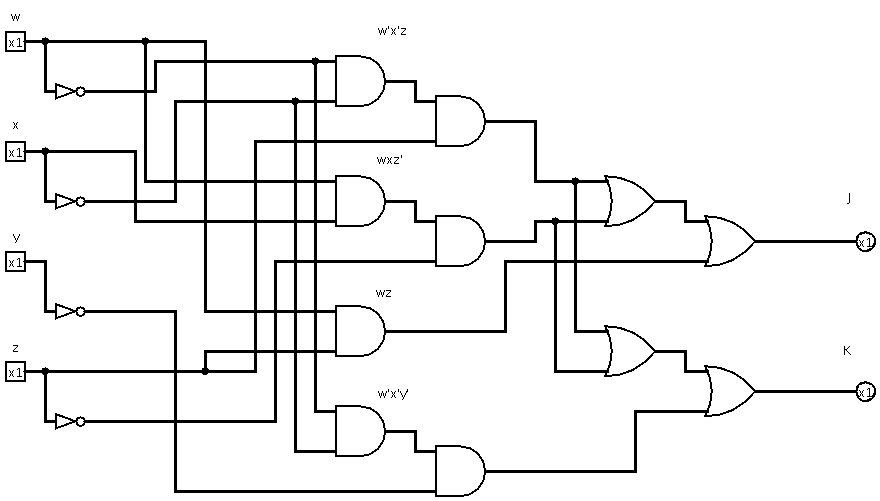
\includegraphics[scale=0.5]{JKjoint-01}
\caption{Circuit diagram of the jointly optimized solution of $J$ and $K$ when limited to two input gates.}
\label{fig:JKjointcircuit}
\end{figure}
4 NOT gates, 7 AND gates and 4 OR gates where used to implement the J and K combined circuit.
(Figure \ref{fig:JKjointcircuit}
\clearpage
\section{Observations}
The results of the implemented circuit in Figure 7 lines up with the Truth Table and produces the expected results.
\begin{table}[!htb]
\center
\begin{tabular}{cc}
\begin{tabular}{lll}
\multicolumn{3}{c}{\bf{$J$ by itself}} \\
gate type & \# gates & \# inputs\\
\hline
AND & 2 & 4\\
OR & 1 & 2\\
NOT & 1 & 1 \\
\hline
\bf{TOTAL} & 4 & 7
\end{tabular}
&
\begin{tabular}{lll}
\multicolumn{3}{c}{\bf{$J$ and $K$ independently}} \\
gate type & \# gates & \# inputs\\
\hline
AND & 8 & 16 \\
OR & 3 & 6 \\
NOT & 5 & 5 \\
\hline
\bf{TOTAL} & 16 & 27
\end{tabular}
\\
\\
\begin{tabular}{lll}
\multicolumn{3}{c}{\bf{$K$ by itself, 2 input gates}} \\
gate type & \# gates & \# inputs\\
\hline
AND & 6 & 12 \\
OR & 2 & 4 \\
NOT & 4 & 4 \\
\hline
\bf{TOTAL} & 12 & 20
\end{tabular}
&
\begin{tabular}{lll}
\multicolumn{3}{c}{\bf{$J$ and $K$ jointly}} \\
gate type & \# gates & \# inputs\\
\hline
AND & 7 & 14 \\
OR & 4 & 8 \\
NOT & 4 & 4 \\
\hline
\bf{TOTAL} & 15 & 26
\end{tabular}
\end{tabular} % outer formatting table
\caption{Metrics of gate and input counts for various configurations
of $J$ and $K$.}
\label{tbl:counts}
\end{table}
\section{Conclusion}
The lab was a success in demonstrating that shared hardware can be used to implement seperate expressions and still produce the desired outcome.
% flush all the figures
%\clearpage
% Uncomment these if you have references,
%\pagebreak
%\renewcommand*{\refname}{\vspace{-8mm}}
%\section{References}
%%\bibliographystyle{plain}
%%\bibliographystyle{mslapa}
%\bibliographystyle{ieeetr}
%\bibliography{../references}
% Appendix (if needed)
\end{document}
% vim:foldmethod=marker
